
% Materials and Methods
%6. Summary of Publication Recommendations
%Published reports must contain sufficient detail to allow other
%experimenters to try to replicate the reported results and to help
%explain failures of replication. Given the limited space that journals
%provide, recommendations will be summarized below for both
%necessary and optional recording and environmental procedures to
%be reported in publications of studies using EDA.
%First and above all, the method of measurement has to be specified:
%endosomatic or exosomatic, direct or alternating current (if
%any) applied to the skin, and constant voltage or constant current.
%The applied voltage (or current) must be noted. If commercially
%available instrumentation has been used, the manufacturer and
%instrument type should be mentioned. Furthermore, calibration
%procedures should be specified.
%Second, methods of signal conditioning and storage need to be
%specified, including procedures for separating EDL from EDRs,
%if applied, time constants of amplifiers, separate grounding procedures,
%if used, A/D conversion rate, and sampling frequency
%(for EDL and EDRs if stored separately).
%Third, recording sites should be specified for active and inactive
%electrodes (if applicable). If the sites were pretreated, the procedure
%should be reported in detail. Also essential is providing details for
%electrodes and electrolytes that were used, such as electrode metal
%(e.g., sintered Ag/AgCl), area of contact (either in square centimeters
%or diameter), method of fixation (e.g., double-sided adhesive
%tape), details of the used electrolyte, such as type of gel or base,
%ionic type and concentration (e.g., 0.08 M or 0.5% NaCl), or, in the
%case of disposable electrodes, brand and type plus as much of the
%above mentioned information as is available from the manufacturer. It is important to know how long electrodes were attached
%before the recording started and how long they stayed in place.
%Details of how polarization was controlled and how electrodes
%were stored should be given if available. In the case of DC recording,
%we recommend using a polarity reversal switch between segments
%within a session.
%Fourth, signal evaluation needs to be reported in detail, whereas
%the sampling rate (for tonic and phasic measures separately, if
%different) and specification of time windows for tonic and phasic
%measures (e.g., latency windows for EDR onset being 1–4 s after
%stimulus onset) are mandatory. For EDRs, a minimum amplitude
%criterion must be specified and reported (e.g., 0.01 mS for SCRs to
%be scored). The standard terminology mentioned in Section 3
%should be adhered to. The term EDR magnitude should be reserved
%for the average amplitude calculated from a series of responses that
%include zero amplitudes. Any treatment of superimposed EDRs
%should be specified. Methods of detection and elimination of
%recording artifacts should be described if applicable.
%Besides the usual details to be reported about procedures for
%laboratory and field settings, it is important for EDA measurement
%to specify baseline conditions in detail, including length and statistical
%treatment during EDAdata evaluation. The gender, age, and
%ethnicity of the participants (e.g., number, range or mean, and
%standard deviation) are essential for comparison with EDA results
%from other studies. Medication or drug use (including caffeine
%intake before participation in the study) need to be reported as well.
%Clothing as well as inside and outside temperatures and their possible
%changes during the recording periods should be reported in as
%much detail as possible. If available (e.g., in case of room airconditioning),
%relative humidity should be reported as well.

\section{Materials}
% mention the SNNU and the lab where the study takes place
All experiments and measurements were conducted within the facilities of Systems Neuroscience and Neurotechnology Unit, especially the Green Lab, which is located at the Saarland University Hospital. 

\subsection{Participants}

\subsection{System Components}
%In this section all the components that are necessary to run the virtual reality system are described.
% It is to mention that the used parts were primarily selected in regard to their availability and the system as a whole was kept as cost-efficient as possible. The system can therefore be very appealing to a variety of users, in need of a low-budget treatment system, suited to be operated in limited spaces.
The virtual reality system is comprised of a number of components, some of which were created in the scope of a different thesis\footnote{This is a reference to the master thesis of Santhosh Nayak, a fellow student, contributing to the project.}. Therefore, this section will focus on components that were built in the scope of the present thesis and delineate what is necessary to run the virtual reality system.
  
\subsection{Hardware}\label{Hardware}
\subsubsection{HTC Vive}
The Vive is a commercial virtual reality system that has been developed by HTC in cooperation with Valve and is composed of a Head-Mounted Display (HMD), a tracking system, called Lighthouse, and two controllers. Inside the virtual environment, which is presented to the user via the HMD, the user's position is tracked by the Lighthouse-System at all times, allowing for the user to explore the virtual environment. The Tracking system is composed of a minimum of two base stations, which are located at the edge of the intended tracking area, approximately 2m above the ground. In addition the controllers can be used to perform tasks and to interact with objects inside the virtual world. The Vive can be used in combination with a any computer fitting the following minimum requirements. 
  
\textbf{System Requirements}
\begin{itemize}
\item Graphics: NVIDIA GeForce™ GTX 1060 or AMD Radeon™ RX 480, equal or higher
\item CPU: Intel™ Core™ i5-4590 or AMD FX™ 8350, equal or higher
\item RAM: minimum of 4 GB RAM
\item Video port: 1x HDMI 1.4-port or DisplayPort 1.2 or newer
\item USB ports: 1x USB 2.0-port or newer
\item Operating System: Windows™ 7 SP1, Windows™ 8.1 or newer or Windows™ 10
\end{itemize}

\textbf{Tracking Space Requirements}\\[10pt]
To guarantee a satisfying experience a minimum room size of 2m x 1.5m with a maximum distance of 5m between base stations is suggested by the manufacturer. 
% descibe calibration , room measurement, visible barrier ,Das Chaperone-System warnt Sie über die Grenzen Ihres Spielbereichs, sodass Sie in VR eingetaucht bleiben können, ohne sich über die reale Welt Gedanken zu machen. 
\subsubsection{BITalino}
The BITalino (r)evolution Plugged kit is an innovative low-cost toolkit that was developed for rapid prototyping of wearable devices and biomedical signal acquisition. The main board, or BITalino Core, is comprised of for major components, the Microcontroller (MCU) Block, the Bluetooth Block, the Power Block with the device's own LiPo battery and the UC-E6 connectors. The MCU features 12 ports, which are divided into 8 analog and 4 digital ports. Of the 7 separately included BITalino sensors, which are connected via cable, only the EDA sensor and the ECG sensor were used. The data is recorded with one of the 4 preset sampling rates and then sent to the user's computer, via a Bluetooth connection. The BITalino is supported by a number of platforms, such Matlab and Unity, allowing for easy implementation in almost any data acquisition process.\\

\textbf{Specifications}
\begin{itemize}
\item Analog Ports: 4 in (10-bit) + 2 in (6-bit) + 1 auxiliary in (battery) + 1 out (8-bit)
\item Digital Ports: 2 in (1-bit) + 2 out (1-bit)
\item Sampling Rate: 1, 10, 100 or 1000Hz
\item Communication: Bluetooth
\item Sensors: ECG, EDA
\item Size: 100x65x6mm
\item Power Supply: LiPo battery (500mA, 3.7V)
\end{itemize}

\textbf{Accessories}
\begin{itemize}
\item 1x EDA Sensor
\item 1x ECG Sensor
\item 1x 3-lead cable
\item 1x 2-lead cable
\item 2x UC-E6 to UC-E6 sensor cable
\item pre-gelled electrodes
\end{itemize}

\subsubsection{VR Unit (VRU)}
VRU is the expression given to the computer, which is used to run the Unity software and power the HMD while the system is in use. It is to mention that the performance of the HTC Vive, in some degree, is reliant on the CPU and GPU of the VRU. Therefore exceeding the minimum requirements, although involving higher cost, has proven to beneficial for the user experience, especially when the used virtual environment relies on realistic real-time lighting effects. On a monitor, which is connected to the VRU, the virtual world, as perceived by the HMD, is displayed for the user to see. However, while the system is in use, the software that is run on the VRU is controlled by a separate computer. Therefore it is essential that the VRU is able to connect to the internet. Alternatively a local network can suffice given one of the following conditions is met:\\[10pt]
a) the CMU (see \ref{CMU}) is located in the same local network as the VRU\\
b) the functions of VRU and CMU are handled by a single computer\footnote{If this variant is used, a Bluetooth adapter is required to connect to the BITalino device.}\\[10pt]
 
\subsubsection{Control and Measurement Unit (CMU)}\label{CMU}
In the early design phase the CMU was conceptualized as a part of the VRU, but it was then separated in regard to its intended use as a mobile control device, for the therapist to use during therapy. However, in our experiment a Laptop served as CMU. The CMU enables the user to submit orders to the VRU, control the BITalino, as well as to view the preprocessed Data. To find detailed explanations to the functions mentioned above, see \ref{Methods}.

%\subsubsection*{Conclusion}
%In conclusion it can be said that the system at hand certainly is built to perform on a minimum budget but also be applicable to a number of clinical applications, particularly the treatment of phobias
\subsection{Software}
As mentioned in section \ref{CMU} the data acquisition is handled by a separate computer. However, all programs were designed to function on any device, capable of running the software in this section. 

\subsubsection{Unity}
Unity is a game development platform, which can be used to create high-quality 3D games and deploy them across a variety of platforms, mobile phones, tablets and desktop computers. The user is enabled to directly target a VR device through the implemented Unity VR Software Development Kits (SDK). The VR environment is built by creating game objects, such as structures and lights, and placing them inside a three dimensional virtual space or importing prefabricated assets from the Asset Store. Each game object can be equipped with a number of components to fit the user's needs. One of the most important aspects to the Unity platform is its scripting API giving the user control over the game environment . This is accomplished by C\# scripts, which are created in Visual Studio 2017 and then attached to the  specific game objects. As a game development platform Unity naturally is provided with an extensive networking environment, including UDP and TCP/IP for communication with external devices. In addition the support, offered to the user in form of the Unity Manual and Scripting API as well as the Asset Store, is sufficient to allow even non-professionals to create their own projects.

\subsubsection{Matlab}
Matlab is a software, which was created to solve mathematical problems. It is used for data acquisition and processing as well as feature extraction from the measured signals.
  
  

\subsection{Virtual Environment}
We have designed our virtual height situation around the concept of a closed room featuring a descending floor. A design, which has been chosen specifically over past approaches for a number of reasons. 
   

\subsection{Virtual Reality Exposure}
To display the virtual environment, a powerful computer(Intel(R) Core(TM) i7-3770, 3.4 GHz and 8 GB RAM) and an Nvidia GeForce GTX 1080 graphics card with 8 GB of dedicated memory (GDDR5X) were used in combination with the HTC-Vive Head-Mounted Display (HMD). The Dual AMOLED displays (3,6" diagonal) of the HMD provided for a high-resolution presentation of the virtual world, with 1080x1200 pixel on each eye. The distance between the pupils was manually adjusted for each participant by means of a knob on the HMD. The Lighthouse Tracking-System, created by the company Valve, allowed to track participant's motion during the exposure in an area of maximal 5 by 5 meter and to project their movement in the virtual environment. The Tracking-System consisted of two stationary sensors, positioned in opposing corners at a height of roughly 2 m, and all the sensors, which were attached to the HMD and the controller by HTC. Due to limited space the exposure area was restricted to an area of 3,5 by 3,5 meter. The program, which was used to remotely control the virtual environment, was written with the Matlab software version R2015a. The virtual environment itself was created with Unity version 5.6.1f1 personal. % mention laptop which is used to run the CMU and data presentation
% Bitalino
We chose this device primarily for the convenience of wireless data transmission, higher maneuverability and less distraction for the user. 
By this a therapist is enabled to communicate with the patient inside VR as if he was there himself and improve the therapy.


\subsubsection{Closed Loop Setup}
The setup, which was used to conduct the experiment, is composed of three major components, interacting with each other in a closed loop fashion (see figure \ref{setupImg}). The virtual environment is ran on the VR-Unit (VRU) and presented to the subjects through the HMD. Inside the virtual reality the fear triggering stimulus is applied, causing a sympathetic reaction in the subject. This reaction is measured by the bitalino device, in the form of an ECG and GSR signal, and then sent to the control and measurement unit (CMU) via bluetooth. This data is processed by the CMU and displayed, in real-time, for the user to evaluate. Based on the visual input, provided by the CMU, a decision to alter the virtual environment can be made by the user.  




\begin{figure}[ht]
\centering
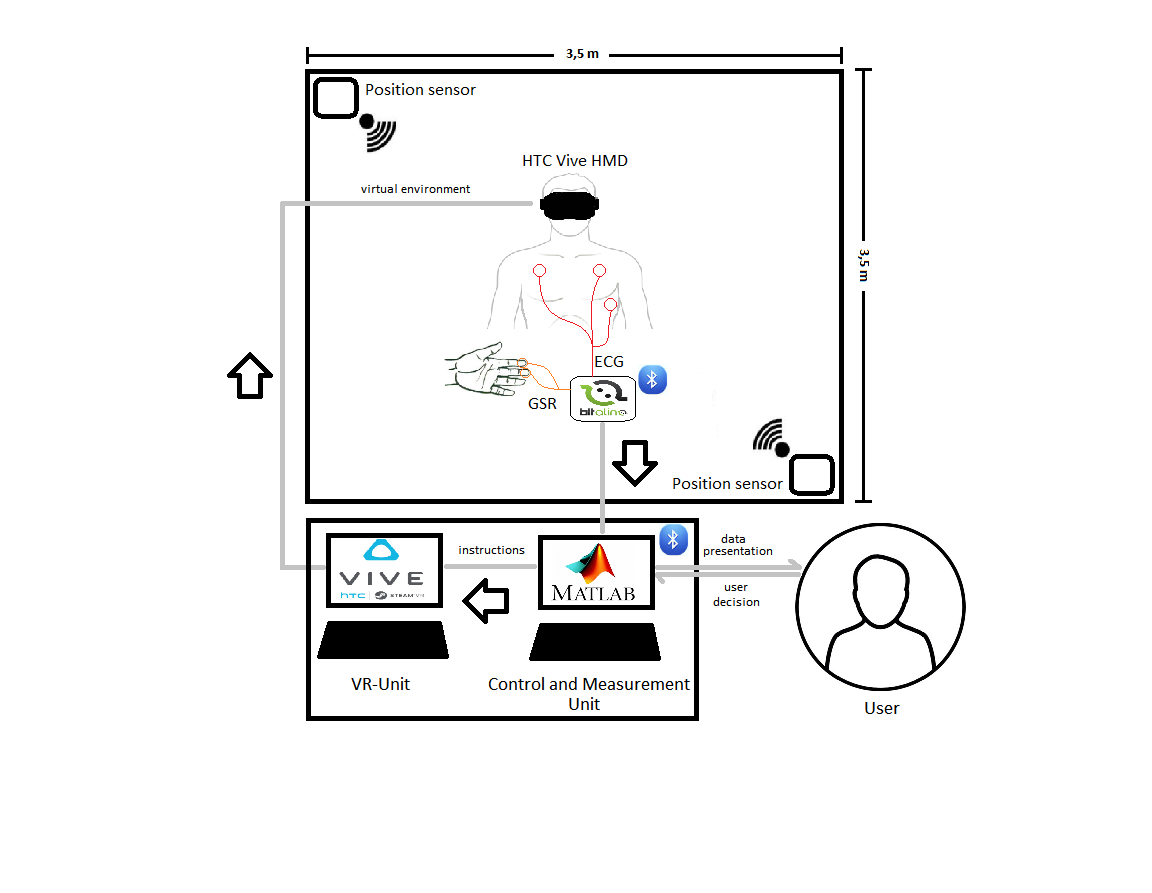
\includegraphics[width=0.8\textwidth]{images/setup.png}
\caption{Closed-loop virtual reality system. The grey line illustrates the closed loop information flow.}
\label{setupImg}
\end{figure}




\section{Methods}\label{Methods}
% methods
- main objective is the measurement of gsr during the therapy and the evaluation of the gsr data concerning the stress of the patient during the therapy\\
- how is the gsr information processed and evaluated?\\
how is it presented to the user?\\
- description of how the VR is controlled by the user(which parameters can be influenced)
- graphic of control chain
\subsection{VR Control}\label{VRControl}
\subsection{Signal Measurement}
\subsection{Signal Processing}
\subsection{Feature Extraction}
\subsection{Procedure}
- how many subjects did participate?\\
- which tasks did the patients fullfill? (cross the bridge etc.)\\
- duration of the experiment\\

- description of the virtual environment, the procedure (baseline measurement,VRET in detail)\\ 
- pictures that show the VE in it's starting state as well as it's therapy state (descended floor)\\
- description of how the VR is controlled by the user(which parameters can be influenced)


-ECG processing frequency domain methods PSD (in task force , reason which method to pick)

\subsubsection{Subject instruction}
Additionally the infrared connection between the base stations of the Lighthouse-System and the HMD should be kept intact at all time
\subsubsection{VR initialization}
%https://docs.unity3d.com/Manual/VROverview.html